\begin{frame}[t]
\frametitle{\charm}
\framesubtitle{}
	\begin{block}{Parallel ...}
		\begin{itemize}[<+->]
		\item \alert<4->{... programming model}
		\item ... programming framework
		\item ... runtime system
	\end{itemize}
	\end{block}
    \begin{itemize}[<+->]
        \item General-purpose
        \item Dataflow
        \item Unified data and task parallelism
        \item Unified handling of shared and distributed memory
        \item Parallel algorithm independent of available processors
        \item Separation of roles and concerns
    \end{itemize}
\end{frame}


\begin{frame}[t]
\frametitle{\charm}
\framesubtitle{}
	\begin{block}{Parallel ...}
		\begin{itemize}
		\item ... programming model
		\item \alert{... programming framework}
		\item ... runtime system
	\end{itemize}
	\end{block}
    \begin{itemize}[<+->]
        \item Code generation, Base classes, utility functions and other API
        \item Multi-paradigm parallel code (procedural, object oriented, generic)
        \item Rich ecosystem of tools
    \end{itemize}
\end{frame}


\begin{frame}[t]
\frametitle{\charm}
\framesubtitle{}
	\begin{block}{Parallel ...}
		\begin{itemize}
		\item ... programming model
		\item ... programming framework
		\item \alert{... runtime system}
	\end{itemize}
	\end{block}
    \begin{itemize}[<+->]
        \item Managed parallel execution
        %\item Shared-nothing by default, explicit sharing for optimization
        \item Measurement-based performance introspection
        \item Adaptive response for better performance
    \end{itemize}
\end{frame}


\begin{frame}
\frametitle{\charm: Some Capabilities}
\framesubtitle{Transparent to application code!}
    \begin{itemize}
        \item Abstracts domain logic from parallel tuning
        \item Seamless parallel composability of modular components
        \item Fault tolerance
        \item Dynamic load balancing
        \item Energy management
    \end{itemize}
\end{frame}


\begin{frame}
\frametitle{\charm: Portability}
{\scriptsize
\onslide<1->{
\begin{block}{\small Environments}
    \begin{columns}
    \begin{column}{0.45\textwidth}
        \begin{itemize}
            \item Embedded ARM: CARMA dev boards, cell phones
            \item Commodity x86: servers, desktops, laptops, tablets
        \end{itemize}
    \end{column}
    \begin{column}{0.45\textwidth}
        \begin{itemize}
            \item Clusters: commodity, with a network
            \item Supercomputers: IBM Blue Gene and POWER, Cray
        \end{itemize}
    \end{column}
    \end{columns}
\end{block}
}
%\only<1>{ 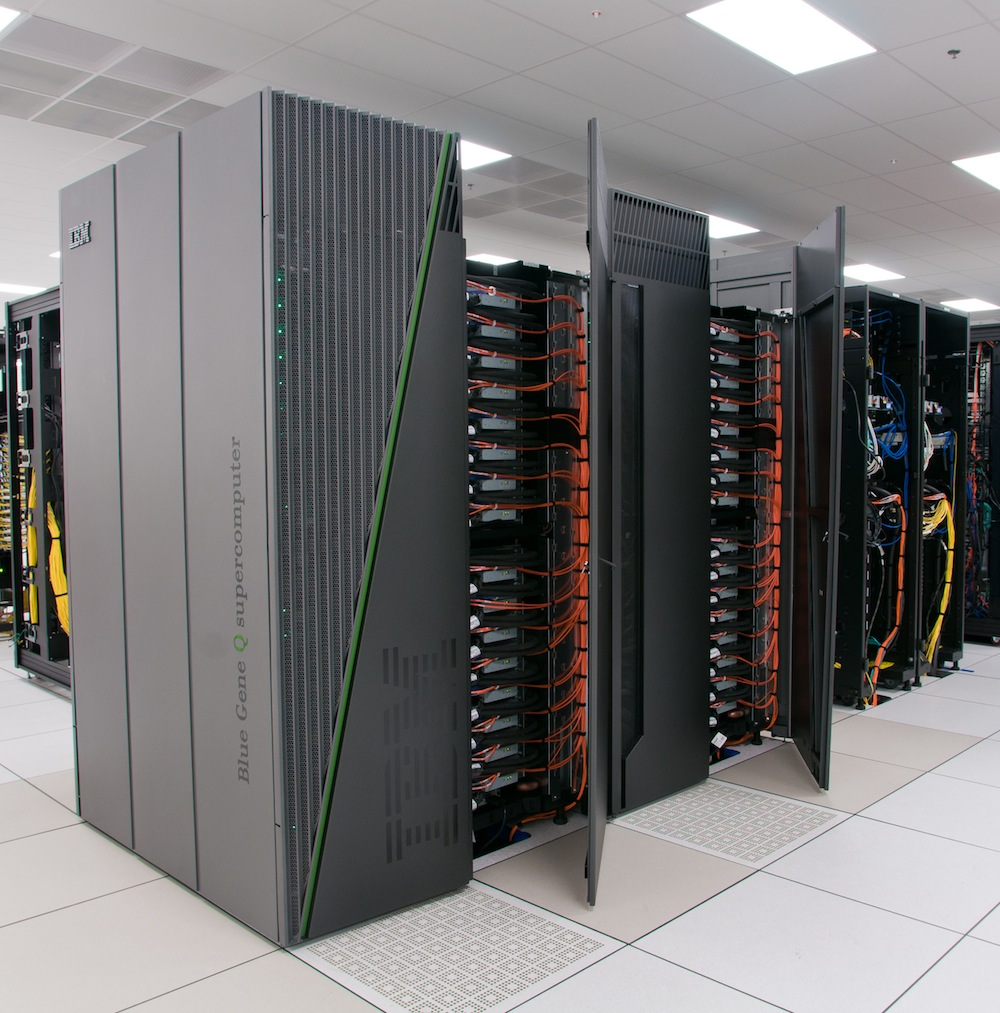
\includegraphics[width=0.48\textwidth]{../figures/mira.jpg} }
\onslide<2->{
\begin{block}{\small Operating Systems}
    \begin{columns}
    \begin{column}{0.45\textwidth}
        \begin{itemize}
            \item Linux
            \item Mac OS X
        \end{itemize}
    \end{column}
    \begin{column}{0.45\textwidth}
        \begin{itemize}
            \item Windows
            \item Proprietary Cray \& IBM
        \end{itemize}
    \end{column}
    \end{columns}
\end{block}
}
%\onslide<3->{
%\begin{block}{\small Network Interfaces}
%    \begin{columns}
%    \begin{column}{0.45\textwidth}
%        \begin{itemize}
%            \item TCP, UDP
%            \item Shared memory
%            \item MPI
%        \end{itemize}
%    \end{column}
%    \begin{column}{0.45\textwidth}
%        \begin{itemize}
%            \item Infiniband Verbs
%            \item IBM BlueGene P,Q (DCMF, PAMI)
%            \item Cray Gemini and Aries (uGNI)
%        \end{itemize}
%    \end{column}
%    \end{columns}
%\end{block}
%}
%\only<1>{ 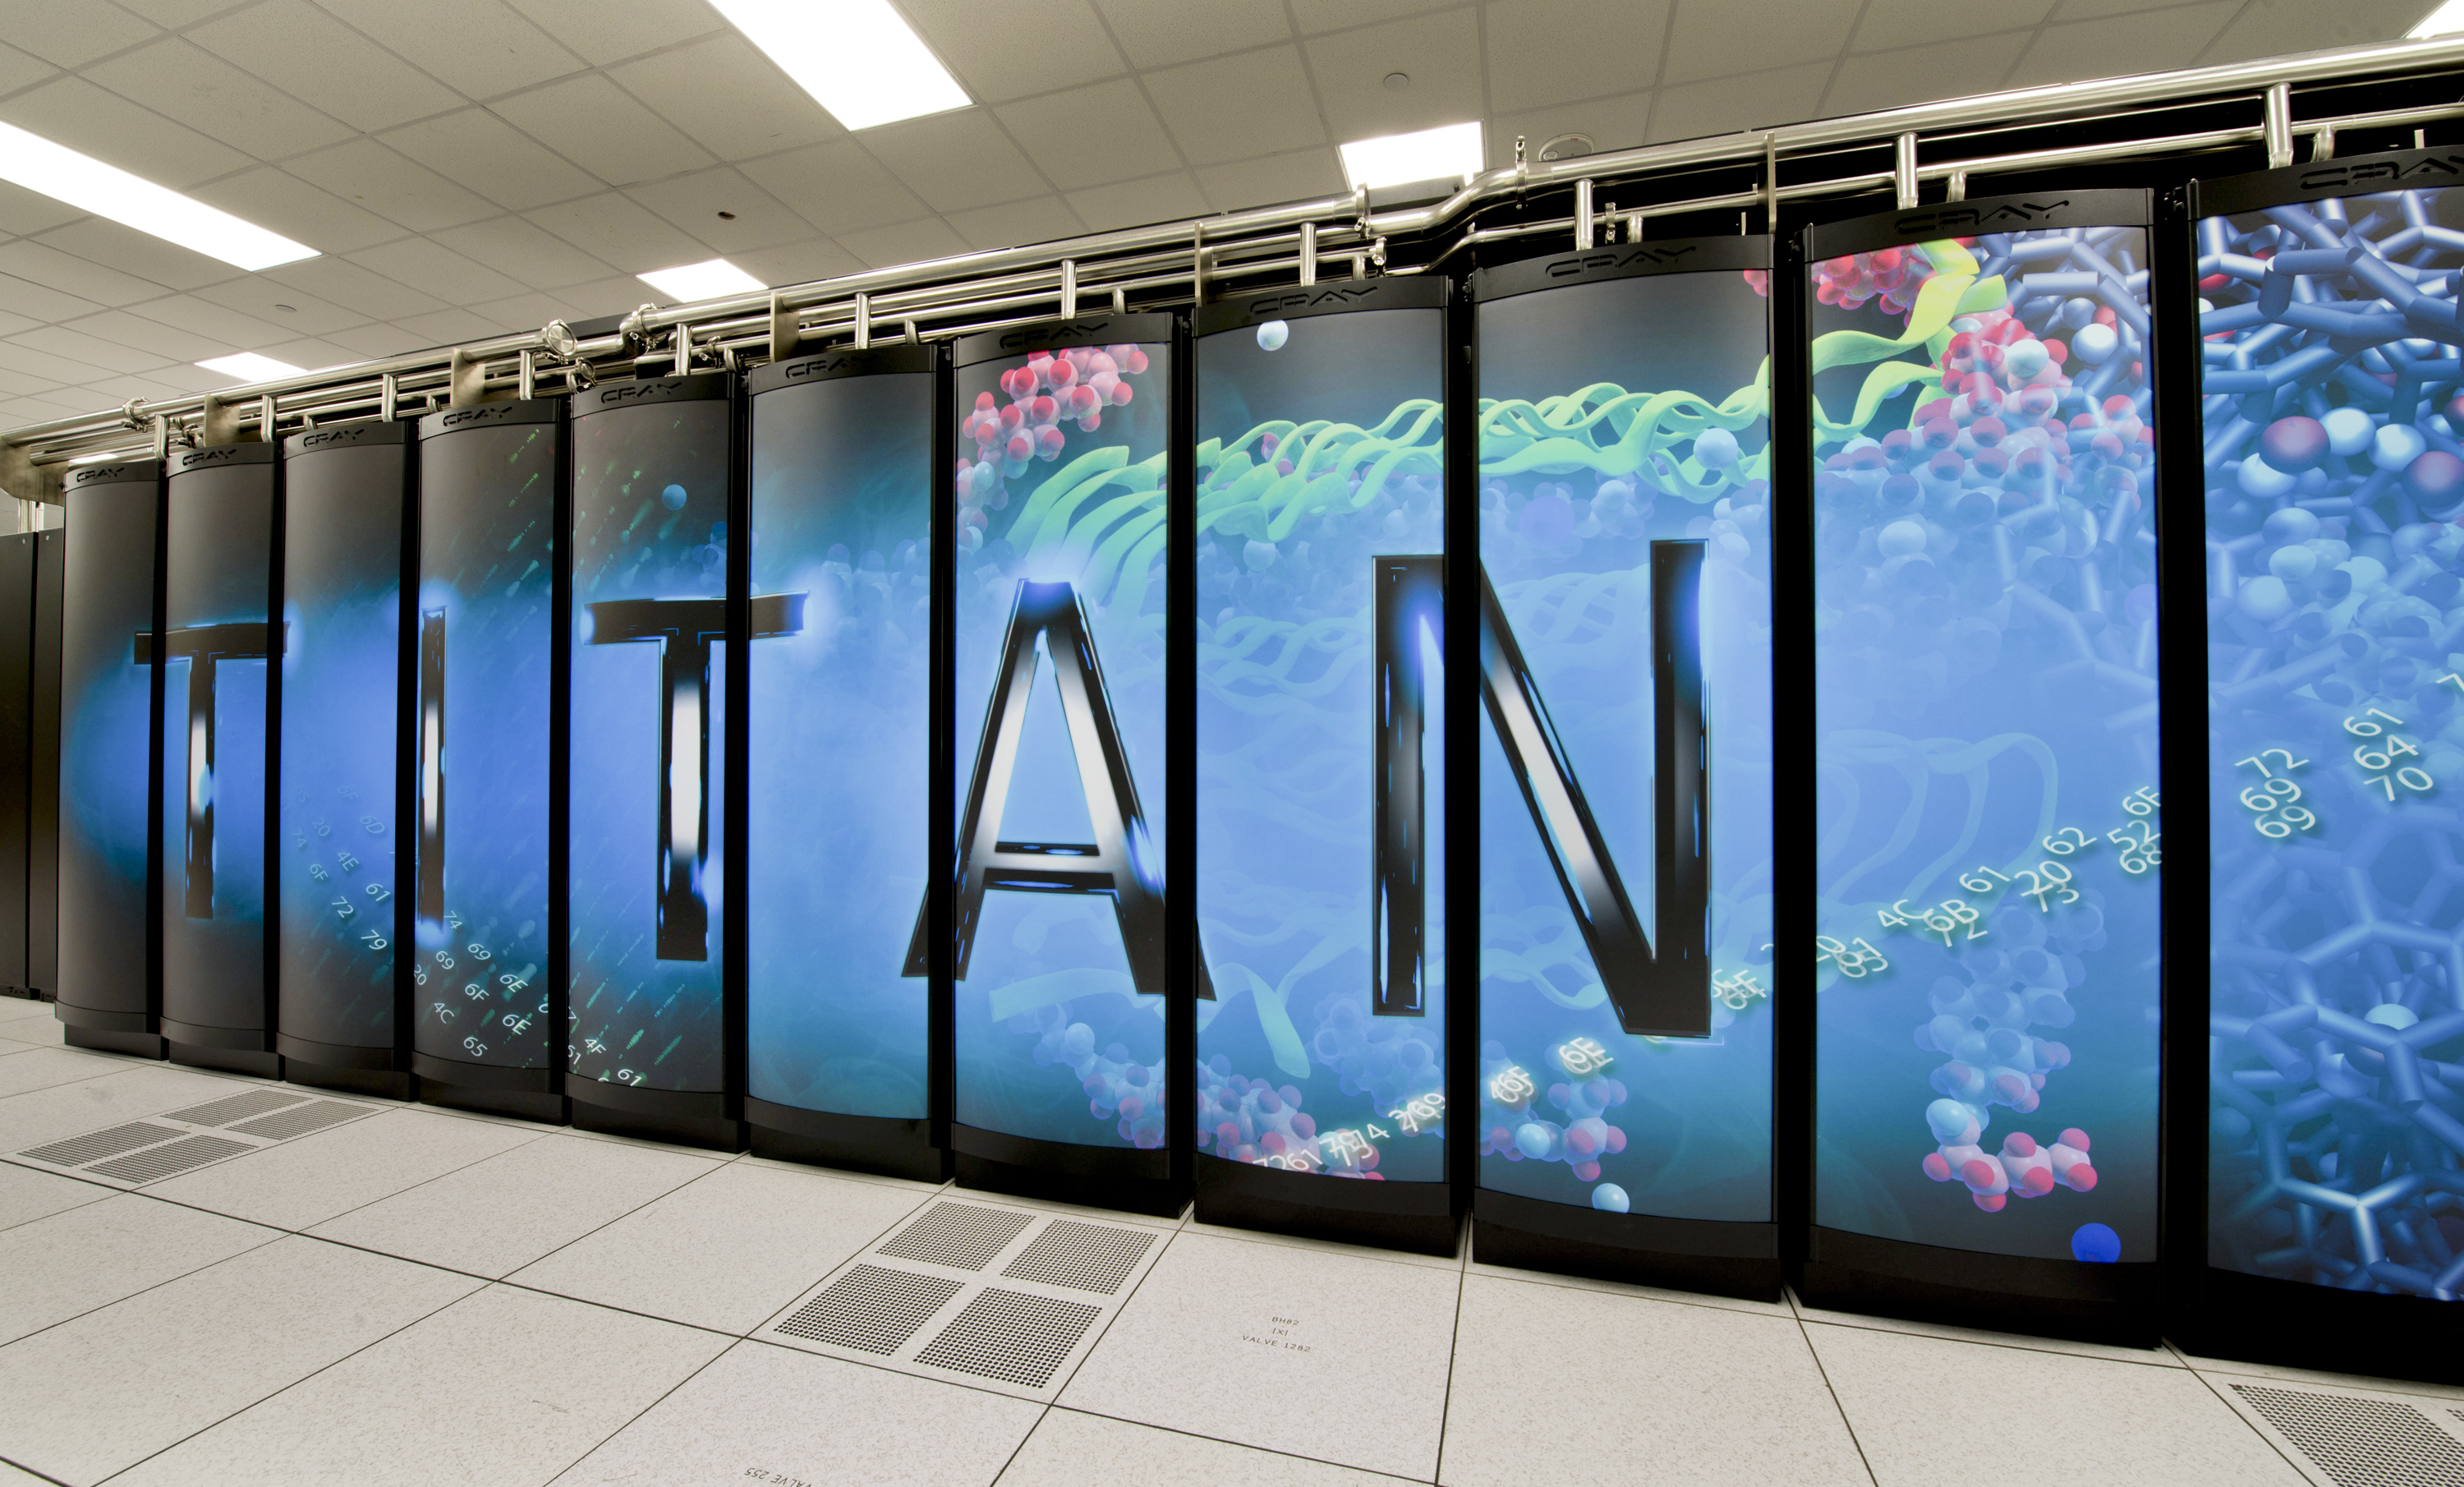
\includegraphics[width=0.48\textwidth]{../figures/titan.jpg} }
\onslide<3->{
\begin{block}{\small Compilers}
    \begin{columns}
    \begin{column}{0.45\textwidth}
        \begin{itemize}
            \item GCC
            \item Clang
            \item Microsoft VC++
            \item IBM XL
        \end{itemize}
    \end{column}
    \begin{column}{0.45\textwidth}
        \begin{itemize}
            \item Intel
            \item Portland Group (PGI)
            \item Cray
            \item Fujitsu
        \end{itemize}
    \end{column}
    \end{columns}
\end{block}
}
}
\end{frame}


\begin{frame}
\frametitle{\charm: Pedigree}
\begin{itemize}
\item Precursors: Rediflow (Keller), Actors, ABCL (Yonezawa)
\item 1987: Chare Kernel arose from parallel Prolog work
\item 1992: Initial C++-based Charm++
\item 1994-1996: NAMD developed
\item 1997: Application-facing abstractions reach near-current form
\item 1997: Adaptive MPI (AMPI) built atop Charm++
\item 2000-present: More applications developed, runtime facilities extended,
  sacling with new machines
\end{itemize}
\end{frame}
